%==================================================================================================================================%
%============================================================= 第二章 预备知识 ====================================================%
%==================================================================================================================================%
\newpage
\chapter{MDE问题} \label{Chap:Basic_Knowledge}
考虑如下问题
\begin{equation}
	\begin{aligned} \frac{\partial q}{\partial s} &=\nabla^{2} q-w q, \quad 0<s \leq f \\ q(\mathbf{r}, 0) &=1 \end{aligned}
\end{equation}

\begin{equation}
1+2=3
\end{equation}
其中w是给定的段。为了具体,令$f=1/2$
\section{二阶方法}

\subsection{Strang分裂方法}
该方法由Rasmussen和Kalosakas提出,表示为$SS^0$,对于空间均匀网格的所有节点r,有:

\begin{equation}
q_{j+1}(\mathbf{r})=\exp \left[-\frac{\Delta s}{2} w(\mathbf{r})\right] \exp \left[\Delta s \nabla^{2}\right] \exp \left[-\frac{\Delta s}{2} w(\mathbf{r})\right] q_{j}(\mathbf{r})
\end{equation}

该方法每步只需要两次FFT,并且具有明显的无条件稳定性。作为一步法,它还允许可变步长,对于平滑的场景,这种方法成本小和且稳定性好,在二阶方案中是其他方法难以比拟的。

然而,它对SCFT计算有一个显着的缺点,它具有较差的高模态阻尼,特别是对于高度隔离的系统和随机(complex Langevin)模拟。


\subsection{IMEX Runge-Kutta方法}
IMEX RK方法具有优异的稳定性,并且允许容易地改变步长和步长控制。
我们下面介绍Ascher等人推导的(2; 2; 2)方案,我们将其表示为$RK_{222}$,而MDE问题可以写为
\begin{equation}
\begin{array}{l}{\left[1-\gamma \Delta s \nabla^{2}\right] q^{(1)}(\mathbf{r})=[1-\gamma \Delta s w(\mathbf{r})] q_{j}(\mathbf{r})} \\ {\left[1-\gamma \Delta s \nabla^{2}\right] q_{j+1}(\mathbf{r})=[1-\beta \Delta s w(\mathbf{r})] q_{j}(\mathbf{r})+\Delta s\left[(1-\gamma) \nabla^{2}-(1-\beta) w(\mathbf{r})\right] q^{(1)}(\mathbf{r})}\end{array}
\end{equation}
其中$\alpha=(2-\sqrt{2})/2$且$\beta=1-1/2\gamma$,这是一个两阶段对角隐式RK(DIRK)方法,每步花费4次FFT便可以实现。



\section{四阶方法及以上}
简单介绍一下四阶IMEX多步法的特点,它每步成本的花费很有效率,每步只需要两次FFT,但是它具有有限的稳定性。

\subsection{四阶外推Strang分裂方法($SS^1$)}
下面介绍四阶外推Strang分裂方法,我们将其表示为$SS^1$,如下:
\begin{equation}
q_{j+1}(\mathbf{r})=\frac{4 S_{\Delta s / 2}^{0}[w] q_{j}(\mathbf{r})-S_{\Delta s}^{0}[w] q_{j}(\mathbf{r})}{3}
\end{equation}
其中$S_{\Delta s}^0[w]q_{j}(r)$代表(1.1.1)的右侧。该方法每步需要6次FFT.通过在$S_{\Delta s/2}^0[w]q_{j}(r)$的计算中组合相邻的半步,可以节省一个w指数。原则上,可以通过对对原始的SS方案应用外推$p-1$次获得阶数为2p的方法。例如应用外推两次得到六阶方案$(SS^2)$:
\begin{equation}
q_{j+1}(\mathbf{r})=\frac{16 S_{\Delta s / 2}^{1}[w] q_{j}(\mathbf{r})-S_{\Delta s}^{1}[w] q_{j}(\mathbf{r})}{15}
\end{equation}
其中$S_{\Delta s}^1[w]q_{j}(r)$代表(1.2.1)的右侧。
这种外推的缺点是特别昂贵,6阶方法每步的成本为18次FFT;并且这两种外推继承了$SS^0$的不良阻尼。



\section{谱延迟校正(SDC)}
由于在等间距节点处重复的数值分布和插值(假设步长均匀),经典的递推修正方法在数值上是不稳定的,并且实际上只能使用非常少量的节点。

于是,Dutt,Greengard和Rokhlin [10]提出了一种新的SDC方法,不但可以克服以上问题,而且可以实现任意高阶,

具体而言,我们现在描述针对MDE特定情况的SDC方法。
重写(1.0.1):
\begin{equation}
q(s, \mathbf{r})=q(0, \mathbf{r})+\int_{0}^{s}\left[\nabla^{2} q(\tau, \mathbf{r})-w(\mathbf{r}) q(\tau, \mathbf{r})\right] d \tau
\end{equation}
定义残差:
\begin{equation}
\epsilon^{[0]}(s, \mathbf{r})=q(0, \mathbf{r})+\int_{0}^{s}\left[\nabla^{2} q^{[0]}(\tau, \mathbf{r})-w(\mathbf{r}) q^{[0]}(\tau, \mathbf{r})\right] d \tau-q^{[0]}(s, \mathbf{r})
\end{equation}

和误差:
\begin{equation}
\delta^{[0]}(s, \mathbf{r})=q(s, \mathbf{r})-q^{|0|}(s, \mathbf{r})
\end{equation}

然后误差满足积分方程:
\begin{equation}
\delta^{[0]}(s, \mathbf{r})=\int_{0}^{s}\left[\nabla^{2} \delta^{[0]}(\tau, \mathbf{r})-w(\mathbf{r}) \delta^{[0]}(\tau, \mathbf{r})\right] d \tau+\epsilon^{[0]}(s, \mathbf{r})
\end{equation}

现在我们可以用求解(1.3.1)的方法求解(1.3.4),得出误差的近似值$\delta^{[0]}$,得到一个新的校正的近似值:
\begin{equation}
q^{ | 1 ]}(s, \mathbf{r})=q^{(0]}(s, \mathbf{r})+\delta^{[0]}(s, \mathbf{r})
\end{equation}
重复利用以上方法求得:
$\mathrm{q}^{(2]} ; \ldots \ldots ; \mathrm{q}^{[\mathrm{J}]}$
我们用$SDC_{N_s}^J$表示延迟校正J.

如果求解(1.3.1)和(1.3.4)的方法是p阶的并且计算残差的积分的精度是$o(\Delta s)^{m}$,则通过进行J延迟校正获得的精度是:

\begin{equation}
O(\Delta s)^{\alpha}, \quad \alpha=\min \{(J+1) p, m\}
\end{equation}

\subsubsection{使用二阶$RK_{222}$求解(1.3.1)与(1.3.4).}

1.使用可变步长直接应用$RK_{222}$(1.1.2)求解(1.3.1):
\begin{equation}
\begin{aligned}\left[1-\gamma \Delta s_{j} \nabla^{2}\right] q^{(1)}(\mathbf{r})=&\left[1-\gamma \Delta s_{j} w(\mathbf{r})\right] q_{j}(\mathbf{r}) \\\left[1-\gamma \Delta s_{j} \nabla^{2}\right] q_{j+1}(\mathbf{r})=&\left[1-\beta \Delta s_{j} w(\mathbf{r})\right] q_{j}(\mathbf{r}) \\ &+\Delta s_{j}\left[(1-\gamma) \nabla^{2}-(1-\beta) w(\mathbf{r})\right] q^{(1)}(\mathbf{r}) \end{aligned}
\end{equation}

对于$j=0,1, \ldots N_{s}$,现在有$\Delta s_{j}=s_{j+1}-s_{j}$,其中$$
s_{j}=\frac{f}{2}-\frac{f}{2} \cos \left(\frac{j \pi}{N_{s}}\right), \quad j=0,1, \ldots N_{s}
$$为[0,1]上$N_s+1$个Chebyshev节点。

利用$RK_{222}$求误差方程,
$$
\begin{aligned}\left[1-\gamma \Delta s_{j} \nabla^{2}\right] \delta^{(1)}(\mathbf{r}) &=\left[1-\gamma \Delta s_{j} w(\mathbf{r})\right] \delta_{j}(\mathbf{r})+\gamma\left(\epsilon_{j+1}(\mathbf{r})-\epsilon_{j}(\mathbf{r})\right) \\\left[1-\gamma \Delta s_{j} \nabla^{2}\right] \delta_{j+1}(\mathbf{r}) &=\left[1-\beta \Delta s_{j} w(\mathbf{r})\right] \delta_{j}(\mathbf{r})+\Delta s_{j}\left[(1-\gamma) \nabla^{2}-(1-\beta) w(\mathbf{r})\right] \delta^{(1)}(\mathbf{r}) \\ &+\epsilon_{j+1}(\mathbf{r})-\epsilon_{j}(\mathbf{r}) \end{aligned}
$$
其中$j=0,1,...,N_s-1$.


下面我们在一个给定的混合场中比较$SS^1$和$SDC$对于MDE问题的处理。

我们给出$w(r)=9cos(6\pi r/L)$,L=10,$\chi^N \approx40$,空间剖分$N_r=128$.

估计在s=f=1/2处两种方法产生的误差。

1.计算$SDC_{1024}^3$的参考解。下面是(s=f=1/2)处的参考解,及两种方法的谱。
\begin{figure}[ht]
	\centering
	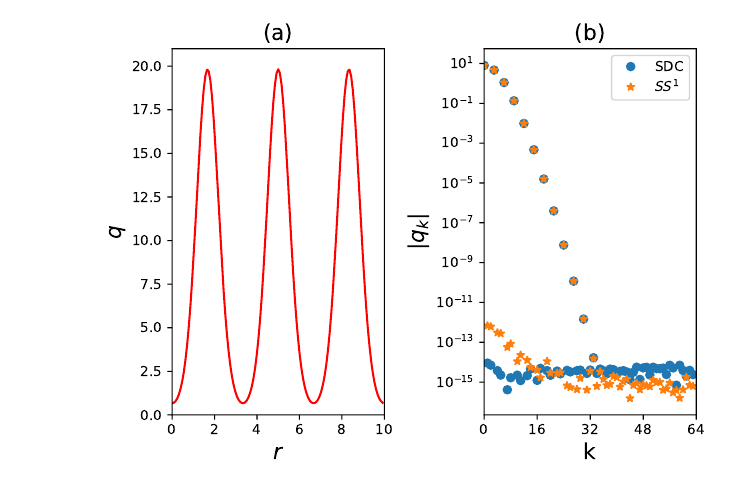
\includegraphics[scale=0.5]{9.png}
	\caption{(a)q(1/2,r),(b)为q(1/2,r)处$SDC_{1024}^3$与$SDC_{1024}^1$的谱,$N_r=128$}
	\label{fig:pathdemo}
\end{figure}

2.使用参考解,评估通过采用$SS^1$和SDC在不同精度水平下获得的近似值的误差。

\begin{figure}[ht]
	\centering
	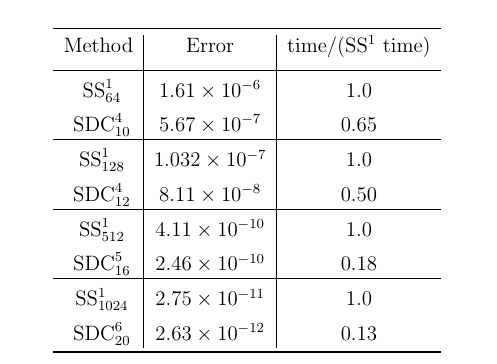
\includegraphics[scale=0.5]{8.png}
	\caption{$SS^1$和SDC对不同精确度的比较.下标是节点数,SDC的上标是延迟校正的次数。$N_r = 256$,使用最大范数计算误差。}
	\label{fig:pathdemo}
\end{figure}

比较可知,SDC方法产生比$SS^1$更精确且更快的近似,且只需要$SS^1$所需节点的一小部分。

\section{轮廓光谱SCFT($SIS$)}
现在考虑二嵌段共聚物溶体的SCFT问题,采用半隐式Siedel鞍点迭代(SIS):
\begin{equation}
\begin{aligned} \frac{\mu_{+}^{j+1}-\mu_{+}^{j}}{\Delta t}=-&\left(g_{A A}+2 g_{A B}+g_{B B}\right) * \mu_{+}^{j+1}+\frac{\delta H\left[\mu_{+}^{j}, \mu_{-}^{j}\right]}{\delta \mu_{+}} \\ &+\left(g_{A A}+2 g_{A B}+g_{B B}\right) * \mu_{+}^{j} \end{aligned}
\end{equation}

\begin{equation}
\frac{\mu_{-}^{j+1}-\mu_{-}^{j}}{\Delta t}=-(2 / \chi N) \mu_{-}^{j+1}-\frac{\delta H\left[\mu_{+}^{j+1}, \mu_{-}^{j}\right]}{\delta \mu_{-}}+(2 / \chi N) \mu_{-}^{j}
\end{equation}

其中*表示卷积,核心的Fourier符号为:
\begin{equation}
\begin{aligned} 
\hat{g}_{AA}(k) &=\frac{2}{k^{4}}\left[f k^{2}+\exp \left(-k^{2} f\right)-1\right] \\ \hat{g}_{A B}(k) &=\frac{1}{k^{4}}\left[1-\exp \left(-k^{2} f\right)\right]\left[1-\exp \left(-k^{2}(1-f)\right)\right] \\ \hat{g}_{B B}(k) &=\frac{2}{k^{-1}}\left[(1-f) k^{2}+\exp \left(-k^{2}(1-f)\right)-1\right] 
\end{aligned}
\end{equation}

我们考虑对称二嵌段f =1/2,$\chi^{N}=16$和$\chi^{N}=80$两种情况来说明。

首先设置鞍点迭代的停止标准,
\begin{equation}
\left|H_{\mathrm{ref}}-H^{j+1}\right|<\epsilon_{H} H_{\mathrm{ref}}
\end{equation}
其中$H_{\mathrm{ref}}$为鞍点处的自由能,$H^{j+1}$是在$\mu_{+}^{j+1}$和$\mu_{-}^{j+1}$处的预估值,$\epsilon_{H}$为精确度。

下面借一个案例来讲解此方法,取$\chi^N=16$,L=10,
SIS的迭代步长为$\Delta t=500$,空间剖分$N_r=256$进行迭代。

图1.3比较了$\chi^N=16$时,$SS^1$和SDC在能量相对误差的不同精度水平。
\begin{figure}[ht]
	\centering
	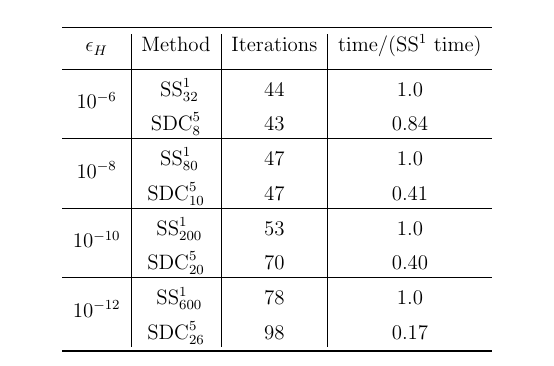
\includegraphics[scale=0.5]{7.png}
	\caption{$\chi^N=16$时,$SS^1$和SDC对于能量的不同精度水平}
	\label{fig:pathdemo}
\end{figure}
\\
\\
\\
每块选择的轮廓点数大约是每种方法达到所需精度所需的最小数量。然而,在SDC方案的情况下,可以使用更少数量的轮廓点,代价是增加迭代次数。在低精度$\epsilon_{\mathcal{H}} \leq 10^{-6}$下,两种方法都具有相似的成本,除了SDC可以使用$SS^1$所需的一小部分轮廓节点,因此存储器要小得多。在更高的精度下,SDC可以轻松胜过$SS^1$并且轮廓点的数量级减少了一个数量级。

但是,SCFT迭代是一种反转平滑算子$\phi_a$和$\phi_b$的方法,因此迭代产生高波数模式的放大,包括舍入误差。

如图1.4所示为400次迭代后$SDC_{128}^6$和$SS_{600}^1$用获得的高精度计算的$\mu_{+}$的光谱:
\begin{figure}[ht]
	\centering
	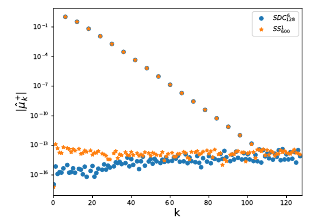
\includegraphics[scale=1]{5.png}
	\caption{$\chi^N=16,L=10$时,$SDC_{128}^6$和$SS_{600}^1$得到的$\mu_{+}$的谱}
	\label{fig:pathdemo}
\end{figure}
我们看到舍入误差有明显的放大,现在是$o(10^{-13})$。

随着$\chi^N$的增加,舍入误差变大更加明显,因为式$-\frac{2}{\chi^N} \mu_{-}$的平滑效应减小。这种现象是针对H的鞍点的反问题的不适定性所固有的,而不是用于解决MDE的特定数值方法,如图1.4所示。如果无人看管,它可能导致精度的显著损失并最终导致迭代的不稳定性,特别是对于大的$\chi^N$。

在一些不适定问题中控制舍入误差增长的一种方法是采用傅立叶滤波器,其包括将所有低于接近机器精度的阈值$\epsilon_F$傅立叶模式设置为零。也就是说,为了计算周期性数组,我们对其进行DFT,将模数小于$\epsilon_F$的所有傅立叶系数设置为零,再作逆变换。


下面我们考虑$\chi^N=80$和$L=5$,空间剖分为$N_r=512$,且SIS的步长为$\Delta t=40$,并在每次迭代时对$\mu_{+}$和$\mu_{-}$应用傅里叶滤波器,阈值$\epsilon_F=10^{-12}$,SIS迭代的初始猜测为:

$\mu_{+}(r)=-0.1 \cos (4 \pi r / L), \quad \mu_{-}(r)=0.1 \cos (4 \pi r / L)$

得到
\begin{figure}[ht]
	\centering
	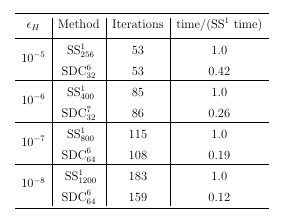
\includegraphics[scale=1]{6.png}
	\caption{$\chi^N=80,L=5$时,$SS^1$和SDC对于能量的不同精度水平}
	\label{fig:pathdemo}
\end{figure}

\section{自适应阶SCFT迭代($AOSDC$)}
一种通过在迭代期间自适应地改变MDE$\quad$SDC方案的顺序来加速SCFT鞍点计算的策略。该策略来源于多级嵌入,使用通过分层次分辨率构造的初始猜测。

其优点是该方法更有效,r和s保持确定(avoiding interpolation),且只有SDC的阶改变。

策略如下:

1.选择每个块的轮廓点数(e.g.based on $\chi^N$)。

2.使用一级延迟校正(四阶方法)开始SCFT鞍点迭代。直到H的第一个变化的相对变化在两次连续迭代中H的第一次变化值小于阈值$\epsilon_{T}$。

3.将延迟校正的次数增加1,并重复直到收敛到所需的准确度水平或者直到达到允许的延迟校正的最大次数。

此外,定义:
$\left\|\frac{\delta H^{j}}{\delta \mu}\right\|=\left\|\frac{\delta H\left[\mu_{+}^{j}, \mu_{+}^{j}\right]}{\delta \mu_{-}}\right\|+\left\|\frac{\delta H\left[\mu_{+}^{j}, \mu_{-}^{j}\right]}{\delta \mu_{-}}\right\|$

然后,迭代过程中,当$$
\left\|\frac{\delta H^{j+1}}{\delta \mu}\right\|-\left\|\frac{\delta H^{j}}{\delta \mu}\right\|<\left\|\frac{\delta H^{j+1}}{\delta \mu}\right\| \epsilon_{T}
$$时,我们将谱延迟校正的级别增加1。

其中阈值$\epsilon_{T}$取决于所需的精确度,范数用$\lVert .\rVert_{\infty}$。

下面是一个特例,其中$\chi^N$=80,$\epsilon_{T}=0.01$.
\begin{figure}[ht]
	\centering
	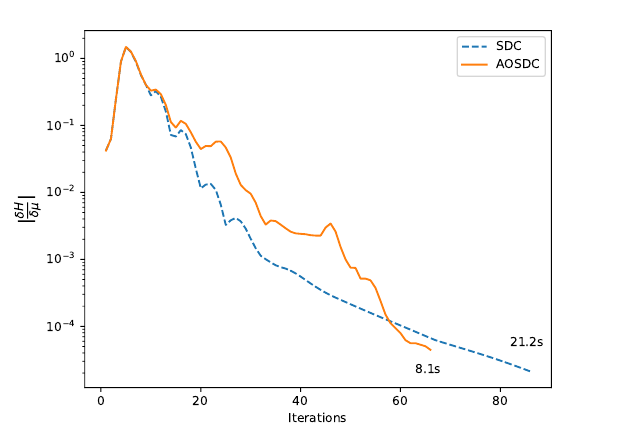
\includegraphics[scale=0.5]{10.png}
	\caption{对于AOSDC和SDC,当$\chi^N=80$时,H随迭代次数的第一次变化的最大范数达到$10^6$的相对能量水平}
	\label{fig:pathdemo}
\end{figure}


对于大多数迭代,AOSDC的误差更大,因为它使用少于7个校正级别;仅在最后4次迭代中,该方法使用的7个校正级别快速达到所需精度。且只花费SDC所需时间的约三分之一。
且大约有12次比$SS^1$更快。
